\documentclass[
  captions=tableheading,
  bibliography=totoc, 
  titepage=firstiscover,
]{scrartcl}

\usepackage{blindtext} %neuer input

\usepackage{longtable} % Tabellen über mehrere Seiten

\usepackage[utf8]{inputenc} %neuer input

\usepackage{scrhack}

\usepackage[aux]{rerunfilecheck} %Warnung falls nochmal kompiliert werden muss

\usepackage{fontspec} %Fonteinstellungen

\recalctypearea{}

\usepackage[main=ngerman]{babel} %deutsche Spracheinstellung

\usepackage{ragged2e} %neuer input

\usepackage{amsmath, nccmath}

\usepackage{amssymb} %viele mathe Symbole

\usepackage{mathtools} %Erweiterungen für amsmath


\DeclarePairedDelimiter{\abs}{\lvert}{\rvert}
\DeclarePairedDelimiter{\norm}{\lVert}{\rVert}

\DeclarePairedDelimiter{\bra}{\langle}{\rvert}
\DeclarePairedDelimiter{\ket}{\lvert}{\rangle}

\DeclarePairedDelimiterX{\braket}[2]{\langle}{\rangle}{
#1 \delimsize| #2
}

\NewDocumentCommand \dif {m}
{
\mathinner{\symup{d} #1}
}


\usepackage[
  math-style=ISO,
  bold-style=ISO,
  sans-style=italic,
  nabla=upright,
  partial=upright,
  warnings-off={
    mathtools-colon,
    mathtools-overbracket,
  },
]{unicode-math}

\setmathfont{Latin Modern Math}
\setmathfont{XITS Math}[range={scr, bfscr}]
\setmathfont{XITS Math}[range={cal, bfcal}, StylisticSet=1]


\usepackage[
  locale=DE,
  separate-uncertainty=true,
  per-mode=reciprocal,
  output-decimal-marker={,},
]{siunitx}

\usepackage[autostyle]{csquotes} %richtige Anführungszeichen

\usepackage{xfrac}

\usepackage{float}

\floatplacement{figure}{htbp}

\floatplacement{table}{htbp}

\usepackage[ %floats innerhalb einer section halten
  section,   %floats innerhalb er section halten
  below,     %unterhalb der Section aber auf der selben Seite ist ok
]{placeins}

\usepackage[
  labelfont=bf,
  font=small,
  width=0.9\textwidth,
]{caption}

\usepackage{subcaption} %subfigure, subtable, subref

\usepackage{graphicx}

\usepackage{grffile}

\usepackage{booktabs}

\usepackage{microtype} %Verbesserungen am Schriftbild

\usepackage[
backend=biber,
]{biblatex}

\addbibresource{../lit.bib}

\usepackage[ %Hyperlinks im Dokument
  german,
  unicode,
  pdfusetitle,
  pdfcreator={},
  pdfproducer={},
]{hyperref}

\usepackage{bookmark}

\usepackage[shortcuts]{extdash}

%\usepackage{warpcol}


\begin{document}
    \title{V703 Das Geiger-Müller-Zählrohr}
    \author{  
    Tobias Rücker\\
    \texorpdfstring{\href{mailto:tobias.ruecker@tu-dortmund.de}{tobias.ruecker@tu-dortmund.de}
    }{}}
    \date{Durchführung: 19.05.2020, Abgabe: 26.05.2020 \vspace{-4ex}}
\maketitle
\thispagestyle{empty}

\newpage
\tableofcontents
\thispagestyle{empty}
\newpage

% Ziel %%%%%%%%%%%%%%%%%%%%%%%%%%%%%%%%%%%%%%%%%%%%%%%%%%%%%%%%%%%%%%%%%%%%%%%%%%%%%%%%%%%%%%%%%%%%%%%%%%%%%%%%%%%%%%%%%%%%%%%%%%%%%%%%%%%%%%%%%%%%%%%%%%%%%%%%%%%%%%%%%%%%%%%%%%%%%%%%%%%%%%%%%%%%%%%%%%%%%%%%%%%%%%%%%

\setcounter{page}{1}
\section{Ziel}\justifying

Das Geiger-Müller-Zählrohr stellt in der Physik ein wichtiges Instrument zur Messung der Intensität
ionisierter Strahlung. Zur näheren Verständnis des Instruments wird im folgenden aus einer 
Messung die Zählrohr-Charakteristik untersucht und die Totzeit des Geräts bestimmt. 

% Theorie %%%%%%%%%%%%%%%%%%%%%%%%%%%%%%%%%%%%%%%%%%%%%%%%%%%%%%%%%%%%%%%%%%%%%%%%%%%%%%%%%%%%%%%%%%%%%%%%%%%%%%%%%%%%%%%%%%%%%%%%%%%%%%%%%%%%%%%%%%%%%%%%%%%%%%%%%%%%%%%%%%%%%%%%%%%%%%%%%%%%%%%%%%%%%%%%%%

\section{Theorie}\justifying

Beim Geiger-Müller-Zählrohr entsteht durch die Absorption von Strahlung ein elektrischer Impuls.
Diese Impulse werden daraufhin durch einen Impulszähler gezählt und damit die Intensität bestimmt.
Der Aufbau des Geiger-Müller-Zählrohrs besteht aus einem Kathodenzylinder in dem sich ein Anodendraht befindet.
Das innere des Zylinders ist mit einem Gasgemisch aus einem Edelgas und einem Alkohol. \cite{V703}
\begin{figure}[H]
    \centering
    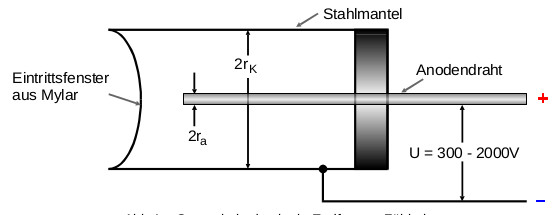
\includegraphics[width=\linewidth]{images/endfenster.jpg}
    \caption{Querschnitt durch ein Endfenster-Zählrohr}
    \label{fig:1}
\end{figure}
\flushleft{Durch\;}\justifying diesen Aufbau können je nach Radiusgröße des Anodendrahts verschiedene 
große Beschleunigungen erreicht werden.
In dem Kathodenzylinder wechselwirken die einkommenden Teilchen mit dem Gas, bis sie
keine Energie mehr besitzen. Dieser Vorgang wird die Primärionisation genannt.
Alle Vorgänge, die danach kommen hängen von der jeweiligen Spannung ab. \cite{V703}
\begin{figure}[H]
    \centering
    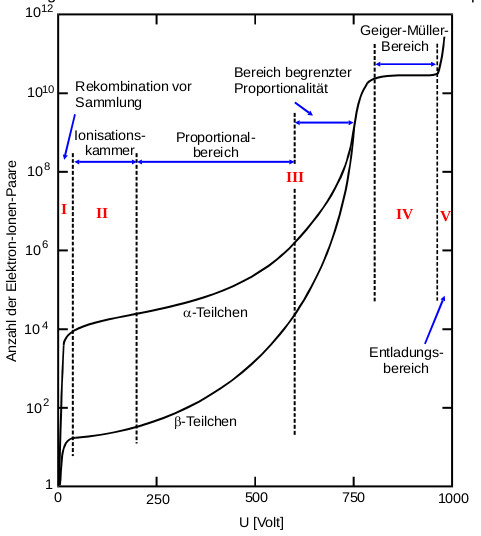
\includegraphics[width=\linewidth]{images/bereich.jpg}
    \caption{Anzahl der erzeugten Elektron-Ionenpaare als Funktion der Spannung }
    \label{fig:2}
\end{figure}
\flushleft{Diese\;}\justifying Graphik veranschaulicht abhängig von der Spannung in welchem Bereich sich das System befindet.
Im ersten Bereich gehen die meisten der durch Ionisation erzeugten Elektronen durch  ist.
verloren. \\
Mit steigender Feldstärke entsteht im Bereich II ein Ionisationsstrom, der proportional zur Energie und Intensität
Dieser Bereich wird Ionisationskammer genannt. Diese stellt eine Vorstufe zum Geiger-Müller-Zählrohr dar.
Hier sind goße Intensitäten nötig, um den kleinen Ionisationsstrom zu messen.\\
In dem dritten Bereich sind die Elektronen energiereich genug, dass die ausgelösten Elektronen
weitere Elektronen ionisieren. Dieser Prozess wird Townsed-Lawine bezeichnet. Hier
ist die Ladung Q im Draht proportional zur Feldstärke und kann als Maß für die
Energie genutzt werden. In diesem Bereich können Intensitäts- und Energiemessungen
vorgenommen werden. Im Allgemeinen wird dieser Bereich als Proportionalitätsrohr bezeichnet.
Der vierte Bereich umfasst den Arbeitsbereich des Zählrohrs. Hier ist die Ladung Q, die im Draht
ankommt, unabhängig von der Primärionisation. 
Ab dem Punkt, wo die $\alpha $- und die $\beta$-Kurve sich überlagern, beginnt der Auslösebereich.
In diesem entstehen UV-Photonen und es finden Elektronenlawinen im gesamten Zählrohr statt.
Hier können nur Intensitätsmessungen vorgenommen werden.
Durch die Ionisationsprozesse bauen die einzelnen Ionen ein elektrisches Feld in der Nähe des
Drahtes auf und schwächen damit die durch die Spannung angelegte Feldstärke. Dadurch finden
keine Elektronenlawinen statt. Dadurch entsteht eine Totzeit wie es in der folgenden Graphik 
zu sehen ist. \cite{V703}
\begin{figure}[H]
    \centering
    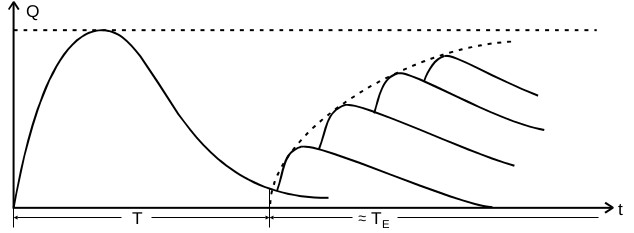
\includegraphics[width=\linewidth]{images/totzeit.jpg}
    \caption{graphische Darstellung der Tot- und Erholungszeit}
    \label{fig:3}
\end{figure}
\flushleft{Nach\;}\justifying der Totzeit kommt eine Erholungszeit, bis die Feldstärke wieder seinen ursprünglichen Wert eingenommen hat.
Die Ionen nehmen dann nach einiger Zeit Elektronen von dem Metall auf. Dabei sind
die Energien der Ionen so groß, dass weitere Elektronen herausgelöst werden.
Dadurch entstehen vereinzelte und versetzte Impulse, welche Nachentladungen
genannt werden. Dabei ist deren Laufzeit größer als die Totzeit, was 
ionisierte Ladungen vortäuscht.
Das ist der Grund, weshalb in dem Gas zusätzlich Alkoholmoleküle sind. Diese
stoßen mit den ionisiertem Edelgas zusammen und werden selbst ionisiert.
Da sie aber eine geringere Energie besitzen, lösen sie keine Sekundärelektronen aus,
sondern regen nur Schwingungen an.\\
In einem Gebiet des vierten Bereichs findet sich die Charakteristik des Zählrohrs.
Das ist der Gebietsteil, in dem ein linearer Teil, welcher Plateau genannt wird, existiert.
Bei einem idealen Gerät findet in diesem Spannungsbereich kein Anstieg statt.
In der Realität exisitieren allerdings noch ein paar Nachentladungen, wodurch ein kleiner 
Anstieg vorhanden ist, wie diese Graphik dies zeigt: \cite{V703}
\begin{figure}[H]
    \centering
    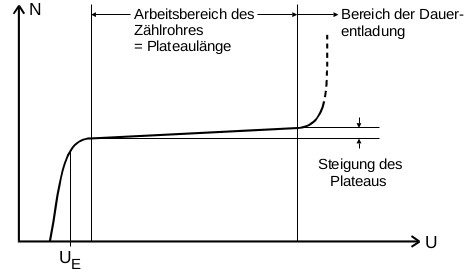
\includegraphics[width=\linewidth]{images/plateau.jpg}
    \caption{Zählrohrcharakteristik(einfallende Strahlung konstant)}
    \label{fig:4}
\end{figure}
\flushleft{Im\;}\justifying fünften und letzten Bereich auf der Graphik \ref{fig:2}
erhöht sich die Anzahl der Nachentladungen drastisch, wodurch es zu einer hohen
Stromdichte kommt, die das Geiger-Müller-Zählrohr zerstören würde.\\
Bei diesen ganzen Messungen muss erkannt werden, wieviele Teilchen in das Volumen vordringen.
Das wird bei den Endfenster-Zählrohren über eine dünnschichtige Wand realisiert, in die
auch $\alpha$-Teilchen eindringen können. Hochenergetische Photonen hingegen haben nur eine 
geringe Chance mit der Wand zu wechselwirken, weshalb Messungen nur bei hohen $\gamma$-Intensitäten
sinnvoll ist.

% Versuchsaufbau + Versuchsdurchführung %%%%%%%%%%%%%%%%%%%%%%%%%%%%%%%%%%%%%%%%%%%%%%%%%%%%%%%%%%%%%%%%%%%%%%%%%%%%%%%%%%%%%%%%%%%%%%%%%%%%%%%%%%%%%%%%%%%%%%%%%%%%%%%%%%%%%%%%%%%%%%%%%%%%%%%%%%%%%%%%%%%%%%%%%%%%%%%%%%%%%%%%%%%%%%%%%%

\section{Versuchsaufbau und Versuchsdurchführung}\justifying
Der Grundlegende Aufbau der Messapartur sieht folgendermaßen aus:
\begin{figure}[H]
    \centering
    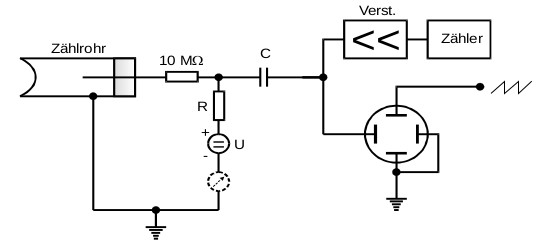
\includegraphics[width=\linewidth]{images/aufbau.jpg}
    \caption{Schematischer Aufbau eines Geiger-Müller-Zählrohrs}
    \label{fig:5}
\end{figure}
\flushleft{Für\;}\justifying die Aufnahme des Charakteristischen Spektrums wird eine $\beta$-Quelle vor das
Fenster des Zählrohrs platziert. Gemessen wird dabei die Zählrate in Abhängigkeit
der Spannung U. Die maximale Impulsrate soll dabei 100 Imp/s nicht überschreiten.
Die Messzeit wird dabei auf einen Wert eingestellt, sodass der statistische Fehler 
geringer als 1\% ist. Die Spannung soll dabei nicht in den Entladungsbereich gehen.
Parallel zu dieser Messung wirdmit einem Amperemeter alle $\SI{50}{\volt} $ die Stromstärke
gemessen.\\
Für die Messung der Totzeit mit dem Oszilloskop soll eine hohe Strahlungsintensität vorhanden sein.
Nun kann, nachdem das Oszilloskop auf die Anstiegsflanke getriggert wurde, die Totzeit
aus dem Graphen gemäß der Abbildung \ref{fig:3} bestimmt werden.\\
Bei der Zwei-Quellen-Methode zur Messung der Totzeit wird zuerst möglichst Präzise die Zählrate des
ersten radioaktiven Präparats bestimmt. Der Aufbau sieht dabei folgendermaßen aus:
\begin{figure}[H]
    \centering
    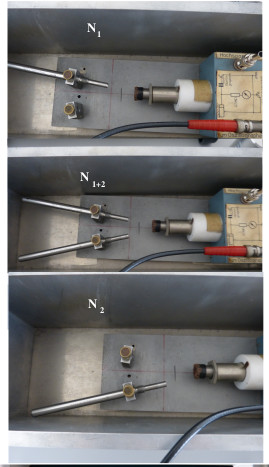
\includegraphics[width=\linewidth]{images/quelle.jpg}
    \caption{Aufbau der Zwei-Quellen-Methode}
    \label{fig:6}
\end{figure}
\flushleft{Im\;}\justifying zweiten Schritt wird wie auf dem mittleren Bild gezeigt eine zweite Quelle in
die Messung eingebracht, ohne die Position der Ersten zu verändern, und dann
erneut die Impulsrate gemessen. Zuletzt wird noch die erste Strahlungsquelle
entfernt und die Zweite alleine gemessen.

% Auswertung %%%%%%%%%%%%%%%%%%%%%%%%%%%%%%%%%%%%%%%%%%%%%%%%%%%%%%%%%%%%%%%%%%%%%%%%%%%%%%%%%%%%%%%%%%%%%%%%%%%%%%%%%%%%%%%%%%%%%%%%%%%%%%%%%%%%%%%%%%%%%%%%%%%%%%%%%%%%%%%%%%%%%%%%%%%%%%%%%%%%%%%%%%%%%%%%%%

\section{Auswertung}

Für diese Auswertung wurde eine $^{204}$Tl-Quelle verwendet. Sie ist so 
platziert worden, dass eine Zählrate con 100 Imp/s nicht überschritten worden ist.
Alle Plots in der Auswertung sind mit matplotlib \cite{matplotlib} erstellt worden und alle Fehler sind mit
uncertainties \cite{uncertainties} berechnet worden.

\subsection{Aufnahme der Charakteristik des Zählrohrs}
Für die Messungen der Charakteristik ist in $\SI{10}{\volt} $-Schritten bei einer 
Integrationszeit von $\SI{60}{\second} $ gemessen worden.
Die Messwerte befinden sich dabei in der folgenden Tabelle:
\input{kenn_table.tex}
\flushleft{Die\,}\justifying Fehler der Anzahl der Zerfälle N sind dabei Poisson verteilt, wodurch jeder Wert 
einen Fehler von
\begin{align}
    \Delta N = \sqrt{N} \label{eq:1}
\end{align}
ergibt.
Für den Graphen ergibt sich dementsprechend:
\begin{figure}[H]
    \centering
    \includegraphics[width=\linewidth]{plot_kenn.pdf}
    \caption{Graph der Kennlinie \cite{matplotlib}}
    \label{fig:7}
\end{figure}

\flushleft{Die\;}\justifying Parameter für die Ausgleichsgerade im Plot sind mit der Funktion polyfit aus SciPy \cite{scipy}
bestimmt worden. Ihre Werte ergeben:
\begin{align}
    N &= aU+b\label{eq:2} \\
    a&= \text{\input{a_kenn.tex}} \label{eq:3} \\
    b&= \text{\input{b_kenn.tex}} \label{eq:4}.
\end{align}
Dabei ist bei der Berechnung der Ausgleichsgeraden nur der Wertebereich des
Plateaus, welcher sich hier von 320-670V erstreckt, berücksichtigt worden.

\subsection{Bestimmung der Totzeit}

Für die Zwei-Quellen-Methode ist eine Totzeit von $\SI{120}{\second} $ eingestellt worden.
Für die drei Zählraten $N_1, N_2$ und $N_{1+2} $ sind die Werte
\begin{align}
    N_1&= \text{\input{N_1.tex}} \label{eq:5} \\
    N_2&= \text{\input{N_2.tex}} \label{eq:6} \\
    N_{1+2}&= \text{\input{N_12.tex}} \label{eq:7} \\
\end{align}
\flushleft{gemessen\;}\justifying worden.
Daraus lässt sich die Totzeit über die Formel \cite{V703}
\begin{align}
    T &\approx \frac{N_1+N_2-N_{1+2}}{2N_1 N_2} \label{eq:8}\\
    T &\approx \text{\input{T.tex}} \label{eq:9}
\end{align}
abschätzen.

\flushleft{Die\,}\justifying Abschätzung der Totzeit über das Oszilloskop wird mit der Abbildung vorgenommen:
\begin{figure}[H]
    \centering
    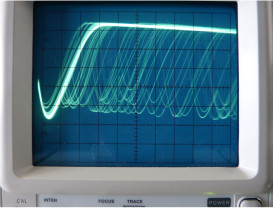
\includegraphics[width=\linewidth]{images/oszi.jpg}
    \caption{Momentaufnahme der Totzeit auf einem Oszilloskop\cite{matplotlib}}
    \label{fig:8}
\end{figure}
\flushleft{Bei diesem\,}\justifying  Bild vom Oszilloskop ist die Zeitachse auf  $\SI{100}{\micro\second}/DIV $
eingestellt.
Für die Zeitkorrektur ergibt sich hieraus ein Wert von
\begin{align}
    T \approx  \label{eq:10} .
\end{align}


\subsection{Pro Teilchen vom Zählrohr freigesetzten Ladungsmenge}

\flushleft{Das\,}\justifying bei der Messung verwendete Amperemeter hat eine Ablesegenauigkeit von

\begin{align}
    \Delta I = \SI{0.05}{\micro\ampere} \label{eq:11}.
\end{align}

\flushleft{Die\,}\justifying Messwerte für die Bestimmung der freigesetzten Ladungsmenge sind in der Tabelle
\begin{table}[H]
\centering
\caption{Messwerte für die Zahl der freigesetzten Ladungen pro eingefallenem Teilchen}
\input{Z_table.tex}
\label{tab:2}
\end{table}
\flushleft{dargestellt}\justifying.
Aus diesen Werten wird die freigesetzte Ladung pro einfallendem Teilchen Z über die Formel \cite{V703}
\begin{align}
    Z= \frac{I}{e_0 N}  \label{eq:12}
\end{align}
berechnet. Hierbei ist $e_0$ die Elementarladung, dessen Wert aus SciPy \cite{scipy} entnommen wird.
In der nachfolgenden Graphik sind die berechneten Z's gegen die Stromstärke aufgetragen.
\begin{figure}[H]
    \centering
    \includegraphics[width=\linewidth]{plot_z.pdf}
    \caption{freigesetzte Ladung pro einfallendem Teilchen Z gegen Stromstärke I\cite{matplotlib}}
    \label{fig:9}
\end{figure}
\flushleft{Die\,}\justifying Ausgleichsgerade ist mit der Funktion polyfit aus SciPy \cite{scipy} erstellt worden.
Die Funktionsparameter zu der Geraden
\begin{align}
    Z &= aI +b \label{eq:13}
    \intertext{
        lauten
    }
    a &= \text{\input{a_Z.tex}} \label{eq:14}\\
    b &= \text{\input{b_Z.tex}} \label{eq:15}.
\end{align}

% Diskussion %%%%%%%%%%%%%%%%%%%%%%%%%%%%%%%%%%%%%%%%%%%%%%%%%%%%%%%%%%%%%%%%%%%%%%%%%%%%%%%%%%%%%%%%%%%%%%%%%%%%%%%%%%%%%%%%%%%%%%%%%%%%%%%%%%%%%%%%%%%%%%%%%%%%%%%%%%%%%%%%%%%%%%%%%%%%%%%%%%%%%%%%%%%%%%%%%%

\section{Diskussion}
Die wichtigsten Werte für die Diskussion sind in der nachfolgenden Tabelle zusammengefasst.
\begin{table}[H]
\centering
\caption{Messwerte}
\begin{tabular}{c c}
    \toprule
    \multicolumn{2}{c}{Messwerte}\\
    \cmidrule(lr{0,5em}){1-2}
    $a_{Plateau}$ & \input{a_kenn.tex} \\
    $b_{Plateau} $ & \input{b_kenn.tex} \\
    $T_{Messung}$ & \input{T.tex}\\
    $T_{Oszi}$ & \\
    \bottomrule
\end{tabular}
\label{tab:3}
\end{table}

\flushleft{Bei\,}\justifying der Messung der Charakteristik ist bewusst darauf geachtet worden, dass
die Impulszahl ungefähr in der Größenordnung von 10000 liegt. Der Grund dafür ist,
dass der statistische Fehler möglichst unter einem Prozent liegen sollte, dafür müssen genug Messungen
vorliegen. Zudem dürfen die Impulse nicht zu hoch sein, da der Alkoholdampf in der
Zylinderkathode begrenzt ist und zu viele Impulse dann zu Nachentladungen führen.
Die Abbildung \ref{fig:7} entspricht der theoretischen Vorstellung der Abbildung 
\ref{fig:4}. Die Steigung ensteht durch die Nachentladungen und zeigt einen
geringen Wert auf, was für einen guten Geiger-Müller-Zähler spricht.
Bei der Auswertung des Graphen für das Plateau sind nicht alle Messwerte 
berücksichtigt worden, da bei den letzen Werten der Übergang zum
fünften Bereich stattfindet und zusätzlich Nachentladungen die Messung
verfälschen. \\
Der Vergleich der Totzeiten von der direkten Messung und dem Oszilloskop zeigt


\flushleft{Die\,}\justifying Abbildung \ref{fig:9} verdeutlicht den erkennbaren linearen Zusammenhang
zwischen der pro Teilchen vom Zählrohr freigesetzten Ladungsmenge und 
der Stromstärke I. Dadurch zeigt sich, wie dominant die Townsed-Lawine sich mit
steigender Stromstärke und gleichzeit steigender Spannung verhält.


% Literatur %%%%%%%%%%%%%%%%%%%%%%%%%%%%%%%%%%%%%%%%%%%%%%%%%%%%%%%%%%%%%%%%%%%%%%%%%%%%%%%%%%%%%%%%%%%%%%%%%%%%%%%%%%%%%%%%%%%%%%%%%%%%%%%%%%%%%%%%%%%%%%%%%%%%%%%%%%%%%%%%%%%%%%%%%%%%%%%%%%%%%%%%%%%%%%%%%%

\newpage
\printbibliography

\end{document}